\documentclass{article}
\usepackage[UTF8]{ctex}
\usepackage[tc]{titlepic}
\usepackage{titlesec}
\usepackage{cite}
\usepackage{fancyhdr}
\usepackage{booktabs}
\usepackage{graphicx}
\usepackage{geometry}
\usepackage{enumitem}
\usepackage[section]{placeins}
\usepackage{listings}
\usepackage{xcolor}

% 设置Python代码样式
\lstset{
	language=Python,
	basicstyle=\ttfamily\small,
	keywordstyle=\color{blue},
	stringstyle=\color{red},
	commentstyle=\color{gray},
	morecomment=[s][\color{magenta}]{\^{}}{\$},
	numbers=left,
	numberstyle=\tiny\color{gray},
	stepnumber=1,
	numbersep=5pt,
	showspaces=false,
	showstringspaces=false,
	showtabs=false,
	frame=single,
	tabsize=4,
	captionpos=b,
	breaklines=true,
	breakatwhitespace=false,
	title=\lstname,
	escapeinside={(*}{*)}
}
\geometry{a4paper,scale=0.8}
\pagestyle{fancy}

\lhead{第 3 次作业\\\today}
\chead{中国科学技术大学\\深度学习导论}

\rhead{Assignment 3\\ {\CTEXoptions[today=old]\today}}
\newcommand{\upcite}[1]{\textsuperscript{\cite{#1}}}

\titleformat*{\section}{\bfseries\Large}
\titleformat*{\subsection}{\bfseries\large}

\title{\bfseries 图卷积神经网络实现节点分类与链路预测}
\author{陈鸿绪 \quad  少年班学院 \quad  PB21000224}
\begin{document}
	\maketitle
	\section*{\centerline{摘要}}
		本此实验完成了利用图卷积神经网络实现在Cora数据集以及citeseer数据集上的节点分类与链路预测。对于数据集划分,本次实验中始终保持训练集、验证集、测试集比例为3:1:1,在经过训练调参工作之后,图卷积模型在Cora测试数据集以及citeseer测试数据集的节点分类准确率高达86.715\%、75.489\%,链路预测的AUC分数高达99.611\%、99.757\%。同时,我们通过变量消融实验探究了自环、层数、DropEdge、PairNorm、激活函数超参数对模型性能的影响。实验训练实验代码位于src文件夹中,代码使用说明具体参见README.md。\\
	
	\setcounter{section}{1}
	\section*{\centerline{一、实验原理}}
	\setcounter{subsection}{0} 
	\subsection{图神经网络}
		图神经网络(Graph Neural Networks,GNNs)的核心思想是通过神经网络学习节点的表示,同时考虑节点的特征和图的结构信息。GNNs 中的每个节点都有一个初始特征向量,这个向量包含了节点的属性信息。图中的边表示节点间的邻接关系。这些关系可以是未加权的,也可以是加权的,表示节点间关系的强度或某种度量。GNNs 通过在节点及其邻居之间传递消息来更新节点的特征表示。这个过程可以看作是节点间的信息聚合,这些聚合函数用于合并邻居节点的特征信息。最后更新函数通过神经网络利用节点自身的特征和聚合后的邻居特征来生成新的节点特征表示。
		
	\subsection{图卷积操作}
		GCNs通过对节点及其邻居的特征信息进行卷积操作来更新节点的表示。这一过程模拟了传统卷积神经网络在图像上的操作,但应用于不规则结构的图数据。GCN 层的公式可以表示为:
		$$H^{(l+1)} = \sigma(\hat{D}^{-\frac{1}{2}}\hat{A}\hat{D}^{-\frac{1}{2}}H^{(l)}W^{(l)})$$
		其中:\(H^{(l)}\) 是第 \(l\) 层的节点特征矩阵,\(W^{(l)}\) 是可学习的权重矩阵,\(\sigma\) 是激活函数,\(\hat{A} = A + I\) 是加入了自连接的邻接矩阵,\(\hat{D}\) 是 \(\hat{A}\) 的度矩阵。
	
	\setcounter{section}{2}
	\section*{\centerline{二、实验过程}}
	\setcounter{subsection}{0} 
	\subsection{读取并划分数据集}
	\begin{enumerate}[label=\textbullet]
		\item 
		读取数据,利用torch\_geometric库集成好的数据读取函数读取Cora和citeseer图数据集。
		\item 
		数据集划分,所有类型的任务数据集划分始终有训练集、验证集、测试集比例为3:1:1,在节点分类任务中指的是节点个数,在链路预测中指的是边个数,两者划分分别使用了RandomNodeSplit,RandomLinkSplit。特别地在链路预测任务中理论上边和无边在训练集中需要保持一样的比例(为了保证正负样本均衡性),注意到其实这点RandomLinkSplit在帮我们划分边集的时候已经考虑进入正负样本均衡了。
	\end{enumerate}
	
	\subsection{定义图卷积操作}
	\begin{enumerate}[label=\textbullet]
		\item 
		信息聚合,GCN 层的公式可以表示为:
		$$H^{(l+1)} = \sigma(\hat{D}^{-\frac{1}{2}}\hat{A}\hat{D}^{-\frac{1}{2}}H^{(l)}W^{(l)})$$
		只需要根据上述定义信息聚合函数以及更新函数即可。
		\item 
		规范化,该操作是为了减轻节点度数差异对卷积结果的影响。通过对邻接矩阵进行规范化,可以使得每个节点的特征更新更加公平。
	\end{enumerate}

	
	\subsection{根据任务的不同类型定义不同图卷积网络}
	注意链路聚合与节点分类的损失函数对象完全不能等价,所以构造GCN时两者也需要根据两者设计不同的损失函数对象。
	\begin{enumerate}[label=\textbullet]
		\item 
		对于链路预测的GCN根据图卷积之后输出节点特征之间的内积正负来预测边是正边还是负边(不存在)。
		\item 
		对于节点分类的GCN根据图卷积之后输出节点特征(特征维度改变成类别数)经过softmax得到每个分类的概率。
	\end{enumerate}
	
	\subsection{训练调试网络}
	最后进行模型训练、参数调试和变量消融实验,选出在测试集上指标表现较优的参数作为最终模型超参数。实验中在激活函数类型为tanh时得到的图卷积模型在Cora测试数据集以及citeseer测试数据集的节点分类准确率高达86.716\%、72.481\%,链路预测的AUC分数高达99.610\%、99.757\%
	
	\clearpage
	
	\setcounter{section}{3}
	\section*{\centerline{三、关键代码讲解}}
	\setcounter{subsection}{0} 
	\subsection{数据加载、划分与处理代码}
	\begin{lstlisting}[language=Python, caption=数据加载、划分与处理代码]
	def load_dataset(device, name):
		dataset = torch_geometric.datasets.Planetoid(root=f"../tmp/{name}", name=name)
		return dataset[0].to(device.__str__()), dataset.num_node_features, dataset.num_classes
	
	def process_data(mission_type: bool, data):
		if mission_type == 0:
		# 链路预测任务数据处理
			transform = RandomLinkSplit(is_undirected=True, num_test=0.2, num_val=0.2)
			train_data, val_data, test_data = transform(data)
			pos_edge_index = train_data.edge_label_index[:, 0: int(train_data.edge_label.size(0)/2)] #是单向的
			neg_edge_index = train_data.edge_label_index[:, int(train_data.edge_label.size(0)/2) + 1: ]
			val_pos_edge_index = val_data.edge_label_index[:, 0: int(val_data.edge_label.size(0)/2)] #是单向的
			val_neg_edge_index = val_data.edge_label_index[:, int(val_data.edge_label.size(0)/2) + 1: ]
			test_pos_edge_index = test_data.edge_label_index[:, 0: int(test_data.edge_label.size(0)/2)] #是单向的
			test_neg_edge_index = test_data.edge_label_index[:, int(test_data.edge_label.size(0)/2) + 1: ]
			return [pos_edge_index, neg_edge_index, val_pos_edge_index, val_neg_edge_index, test_pos_edge_index, test_neg_edge_index]
		if mission_type == 1:
		# 节点分类任务数据处理
			transform = RandomNodeSplit(num_test=0.2, num_val=0.2)
			trans_data = transform(data)
			return [trans_data.train_mask, trans_data.val_mask, trans_data.test_mask]
	\end{lstlisting}
	
	 这段代码构造了两个函数,其中一个函数是加载数据集函数;第二个函数是根据数据集进行训练集、验证集、测试集比例为3:1:1的划分,同时
	由于不同任务关注的对象不一样,所以两者需要分别进行不同的数据划分(这里是通过0,1记号来标记不同任务类型),节点预测针对节点划分,而链路预测是针对边划分,边的正负样本平衡性也得到保证。
	
	\subsection{图卷积操作}
	
	\begin{lstlisting}[language=Python, caption=图卷积操作代码]
		class GCNConv(torch.nn.Module):
		
			def __init__(self, in_channel, out_channel, device = 'cuda'):
				super(GCNConv, self).__init__()
				self.in_channel = in_channel
				self.out_channel = out_channel
				self.weight = nn.Parameter(torch.randn(in_channel, out_channel))    
				self.device = device
			
			def __repr__(self):
				return f'GCNConv({self.in_channel}, {self.out_channel})'
			
			def forward(self, x, edge_index):
				g = dgl.DGLGraph().to('cuda')
				g.add_nodes(x.size(0))
				#g = dgl.graph((edge_index[0], edge_index[1])).to(self.device)
				g.add_edges(edge_index[0], edge_index[1])
				g = g.add_self_loop()
				# add自环
				transform = dgl.DropEdge(p = 0)
				# 随机丢弃
				g = transform(g)
				g.ndata['h'] = torch.mm(x, self.weight)
				degs = g.out_degrees().float()  # D
				norm = torch.pow(degs, -0.5)  # D^{-1/2}
				norm[torch.isinf(norm)] = 0
				g.ndata['norm'] = norm.unsqueeze(1)  
				g.update_all(self.gcn_msg, self.gcn_reduce)
				x = nnFun.normalize(g.ndata['h'], p=2, dim=1)
				x = nnFun.relu(x)
				return x
			
			def gcn_msg(self, edge):
				msg = edge.src['h'] * edge.src['norm']
				return {'m': msg}
			
			# 定义消息聚合规则
			def gcn_reduce(self, node):
				accum = torch.sum(node.mailbox['m'], 1) * node.data['norm']
				return {'h': accum}
	\end{lstlisting}
	这段代码利用GCN 卷积层的定义公式进行信息聚合和信息更新函数编写。其中gcn\_reduce函数定义了消息聚合规则。
	
\subsection{链路预测的GCN模型}
	
	\begin{lstlisting}[language=Python, caption=链路预测的GCN模型代码]
	class GCN(torch.nn.Module):
	
		def __init__(self, features, hidden_dimensions: list, classes):
			super(GCN, self).__init__()
			### encode
			layers = []
			channel = features
			for s in hidden_dimensions:
				layers.append((GCNConv(channel, s), 'x, edge_index -> x'))
				channel = s
			layers.append((GCNConv(channel, classes), 'x, edge_index -> x'))
			self.convseq = Sequential('x, edge_index', layers)
		
		
		def forward(self, x, pos_edge_index, neg_edge_index):
			### encode
			reversed_pos_edge_index = pos_edge_index[torch.tensor([1, 0]), :]
			pos_edge_index_mut = torch.cat([pos_edge_index, reversed_pos_edge_index], dim=-1)
			z = self.convseq(x, pos_edge_index_mut)
			### decode
			selected_edge_index = torch.cat([pos_edge_index, neg_edge_index], dim=-1)
			logits = (z[selected_edge_index[0]] * z[selected_edge_index[1]]).sum(dim=-1)
			return logits   
	\end{lstlisting}
	链路预测任务需要传入正边和负边,若干个图卷积之后需要再对传入边集中任意一条边两端点所对应的特征向量做内积,向前传播输出即为传入边集在图卷积后上述内积的列表。

\subsection{节点分类的GCN模型}

\begin{lstlisting}[language=Python, caption=链路预测的GCN模型代码]
	class GCN(torch.nn.Module):
	
		def __init__(self, features, hidden_dimensions: list, classes):
			super(GCN, self).__init__()
			layers = []
			channel = features
			for s in hidden_dimensions:
				layers.append((GCNConv(channel, s), 'x, edge_index -> x'))
				channel = s
			layers.append((GCNConv(channel, classes), 'x, edge_index -> x'))
			self.convseq = Sequential('x, edge_index', layers)
		
		def forward(self, data):
			x = self.convseq(data.x, data.edge_index)
			return nnFun.log_softmax(x, dim=1)
\end{lstlisting}
节点分类的GCN根据图卷积之后输出节点特征(特征维度改变成类别数)经过softmax得到每个分类的概率,每个节点得到一个概率向量,这正是向前传播得到的结果。


	\setcounter{section}{4}
	\section*{\centerline{四、对超参数的调试与结果分析}}
	为了便于探究一些超参数的影响从而进行消融实验,实验中将始终保持某些超参数的不变性。对于节点分类任务与链路预测任务而言,超参数设置如下表所示:
	\begin{table}[!ht]
		\caption{\textbf{节点分类任务的不变参数}}%标题
		\centering%
		\begin{tabular}{ccccccccc}
			\hline
			学习率    & 最大轮数 & decay\_rate & weight\_decay &隐藏层Conv输出特征维数\\ \hline
			0.005     & 1500  &  1  & 5e-4  & 512   \\ \hline
		\end{tabular}
	\end{table}
	
	\begin{table}[!ht]
		\caption{\textbf{链路预测任务的不变参数}}%标题
		\centering%
		\begin{tabular}{ccccccccc}
			\hline
			学习率    & 最大轮数 & decay\_rate & weight\_decay &隐藏层Conv输出特征维数\\ \hline
			0.01     & 400(Cora) 600(citeseer)  &  1  & 5e-4  & 512   \\ \hline
		\end{tabular}
	\end{table}
	
	进行消融实验时,会按照参照标准超参数进行对比实验(即如果没有提到某参数的设置,则默认设置为下面标准值):
	\begin{table}[!ht]
		\caption{\textbf{链路预测任务的不变参数}}%标题
		\centering%
		\begin{tabular}{ccccccccc}
			\hline
			网络层数    & 激活函数 & 自环有无 & DropEdge & PairNorm\\ \hline
			2     & ReLU  &  存在  & 不使用  & 不使用 \\ \hline
		\end{tabular}
	\end{table}
	
	
	\setcounter{subsection}{0} 
	\subsection{探究自环的有无对模型的影响}
	\begin{table}[!ht]
		\caption{\textbf{有无自环条件下模型表现}}%标题
		\centering%
		\begin{tabular}{|l|ll|ll|}
			\hline
			数据集  & \multicolumn{2}{l|}{Cora} & \multicolumn{2}{l|}{citeseer} \\ \hline
			有无自环 & 链路预测(AUC)   & 节点分类(ACC)   & 链路预测(AUC)     & 节点分类(ACC)     \\ \hline
			有  &  96.823\%       &   85.977\%     & 96.225\%             & 71.128\%              \\
			无  &  96.410\%           &   83.210\%          &  97.158\%            & 68.872\%              \\ \hline
		\end{tabular}
	\end{table}
	
	如果图卷积不包含自环,那么在信息聚合过程中,每个节点只能接收其邻居节点的信息,自身的特征信息不会被保留。此时如果网络深度就会影响网络节点特征趋于一致,进行会影响模型性能。在上述表格中,我们注意到对链路预测任务而言,似乎有无自环对模型性能影响并不大,因为模型在两个数据集的指标变化不超过1\%;然而对节点分类任务而言,模型没有自环性能下降严重,在两个数据集上,模型准确率均下降了2-3\%。所以可以看出自环对节点分类任务更加敏感,而对于链路预测任务,我们考察的是节点与节点之间的联系,自然可以直感受到节点内部特征并没有给节点预测带来多少信息量,所以模型表现浮动并不大。
	
	\clearpage
		\subsection{探究激活函数类型对模型的影响}
	
	\begin{table}[!ht]
		\caption{\textbf{不同激活函数类型下模型表现}}%标题
		\centering%
		\begin{tabular}{|l|ll|ll|}
			\hline
			数据集 & \multicolumn{2}{l|}{Cora} & \multicolumn{2}{l|}{citeseer} \\ \hline
			激活函数类型  & 链路预测(AUC)   & 节点分类(ACC)   & 链路预测(AUC)     & 节点分类(ACC)     \\ \hline
			ReLU   &  96.823\%       &   85.977\%     & 96.225\%             & 71.128\%              \\
			LeakyReLU(0.1)  &97.945\%&86.531\%        &96.279\%              &72.781\%              \\
			Tanh   &  99.757\%       &  86.716\%      & 99.611\%            & 69.022\%              \\ \hline 
		\end{tabular}
	\end{table}
	我们由上表可以发现LeakyReLU在测试集上的表现是全部优于普通ReLU的。对于两个数据集上的链路预测任务,Tanh激活函数的表现非常突出,链路预测任务的AUC分数达到了99\%,同时在Cora数据集上的节点分类任务也是top-1,但是可以看见在citeseer数据集上节点分类的表现却不是很理想,结合控制台输出其实这时候模型处于过拟合状态(epoch 1500过大),导致Tanh激活函数模型在测试集上表现明显差于ReLU和LeakyReLU激活函数模型。
	
	\subsection{探究PairNorm对模型的影响}
	\begin{table}[!ht]
		\caption{\textbf{有无PairNorm模型表现(数字后标注的代表epoch减少到)}}%标题
		\centering%
		\begin{tabular}{|l|ll|ll|}
			\hline
			数据集 & \multicolumn{2}{l|}{Cora} & \multicolumn{2}{l|}{citeseer} \\ \hline
			PairNorm  & 链路预测(AUC)   & 节点分类(ACC)   & 链路预测(AUC)     & 节点分类(ACC)     \\ \hline
			不存在   &  96.823\%       &   85.977\%     & 96.225\%             & 71.128\%              \\
			存在   &  96.690\%       &  80.442\%      & 96.342\%            & 69.323\%              \\
			存在   &  96.824\%       &  84.132\%(200 epoch)      & 96.677\%           & 69.473\%(180 epoch)              \\ \hline 
		\end{tabular}
	\end{table}
	根据上述表格,我们发现PairNorm对实验中的浅层图卷积网络似乎并没有指标上质的提升,但是我们发现使用了PairNorm之后模型收敛得到了加快,这点可以从节点分类任务使用的两种不同epoch看出,对于存在PairNorm但是epoch为1500的默认情况,明显发现模型处于过拟合状态(因为此时指标比不存在PairNorm所得指标差别较大,同时控制台输出的验证集上的指标变化也是过拟合特征),然而不存在PairNorm的节点分类任务在epoch为1500时却没有表现出过拟合,这点由表中最后一行指标可以看出,所以存在PairNorm时,模型所需要的epoch大幅度减少,这说明PairNorm可以有效加快训练收敛,但就浅层图卷积网络而言,PairNorm似乎并没有带来指标上的提高。作为一种正则化手段,PairNorm确实有上述加快模型收敛的正则化作用。
	\subsection{探究层数对模型的影响}
	
	\begin{table}[!ht]
		\caption{\textbf{不同网络层数下模型表现}}%标题
		\centering%
		\begin{tabular}{|l|ll|ll|}
			\hline
			数据集 & \multicolumn{2}{l|}{Cora} & \multicolumn{2}{l|}{citeseer} \\ \hline
			层数  & 链路预测(AUC)   & 节点分类(ACC)   & 链路预测(AUC)     & 节点分类(ACC)     \\ \hline
			2   &  96.823\%       &   85.977\%     & 96.225\%             & 71.128\%              \\
			3   &  96.267\%       &  85.608\%      & 97.103\%             & 72.030\%              \\
			5   &  94.915\%       &  83.394\%      & 93.990\%             & 70.827\%          \\ \hline
		\end{tabular}
	\end{table}
	对于Cora数据集节点分类而言,随着网络层数的增加,模型性能基本上没有上升,反而出现了轻微的下降,对于citeseer数据集而言,在网络层数为3时,模型性能最优,网络层数为5时,模型性能小幅度下降。所以可以基本认定对于Cora、citeseer数据集模型深度分别在2层、3层可以达到一个较好的性能,当然理论上而言在一定范围内,模型层数越大,表征能力肯定越强,但是由于相同的参数设定原因,不同层数的网络模型有不同程度的拟合状态,进而理论上的表现并没有得到很好的体现。
	
	\subsection{探究DropEdge对模型的影响}
	
	\begin{table}[!ht]
		\caption{\textbf{不同DropEdge概率下模型表现}}%标题
		\centering%
		\begin{tabular}{|l|ll|ll|}
			\hline
			数据集 & \multicolumn{2}{l|}{Cora} & \multicolumn{2}{l|}{citeseer} \\ \hline
			丢弃概率  & 链路预测(AUC)   & 节点分类(ACC)   & 链路预测(AUC)     & 节点分类(ACC)     \\ \hline
			0   &  96.823\%       &   85.977\%     & 96.225\%             & 71.128\%              \\
			0.1   &  95.854\%       &  82.841\%      & 93.322\%             & 68.721\%              \\ \hline 
		\end{tabular}
	\end{table}
	我们可以看见在概率设置为较小的值0.1时,模型性能就已经出现明显的下降,理论上适当的DropEdge会提高模型的鲁棒性,模型性能会有所提升,但是由于边在图中包含了重要的信息,随机删除边可能会导致一些重要信息丢失,所以即使是较小概率的DropEdge也会给模型带来性能下降。另一方面DropEdge确实可以提升深度图卷积网络在节点分类任务上的性能,但是我们实验对象是只有两层图卷积层,这就意味着DropEdge减弱过平滑的作用就无法有效体现。
	
	\setcounter{section}{5}
	\section*{\centerline{五、选择最佳参数并进行单次训练}}
	根据上述讨论和作者自己的调参测试,最终参数的选择如下表所示,对应的损失曲线也在下面展示。
	\begin{table}[!ht]
		\caption{\textbf{选择参数以及相应指标分数}}%标题
		\centering%
		\begin{tabular}{|l|ll|ll|}
			\hline
			数据集 & \multicolumn{2}{l|}{Cora} & \multicolumn{2}{l|}{citeseer} \\ \hline
			超参数  & 链路预测(AUC)   & 节点分类(ACC)   & 链路预测(AUC)     & 节点分类(ACC)     \\ 
			学习率   &  0.01       &   0.005     & 0.01             & 0.005              \\
			epoch数   &  400       &  1500      & 600            & 400              \\ 
			图卷积层数   &  2       &  2      & 2            & 4             \\
			激活函数  &  Tanh      &  Tanh      & Tanh            & Tanh              \\  
			decay rate & 1       &  1      & 1            & 1              \\ 
			有无自环   &  存在       &  存在      & 存在           & 存在              \\ 
			有无PairNorm  & 不使用       &  不使用      & 不使用            & 不使用             \\ 
			有无DropEdge   &  不使用       &  不使用       & 不使用           & 不使用               \\ 
			评估分数 &AUC: 99.611\% & ACC: 86.715\% & AUC: 99.757\% & ACC: 75.489\% \\\hline
		\end{tabular}
	\end{table}
	 \begin{figure}[h]
		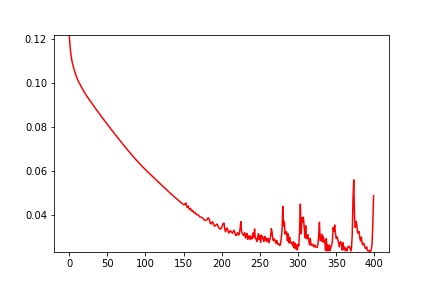
\includegraphics[scale=0.5]{loss-52.png}
		\quad
		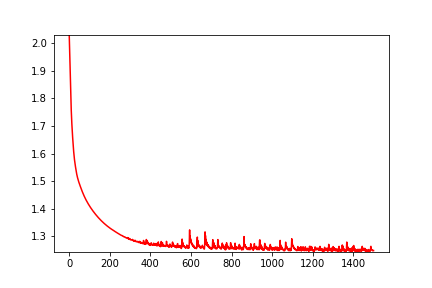
\includegraphics[scale=0.5]{loss-51.png}
		\caption{左图:Cora链路预测loss曲线,右图:Cora节点分类loss曲线}
	\end{figure}
	\begin{figure}[h]
		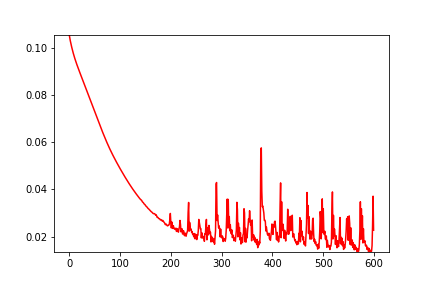
\includegraphics[scale=0.5]{loss-55.png}
		\quad
		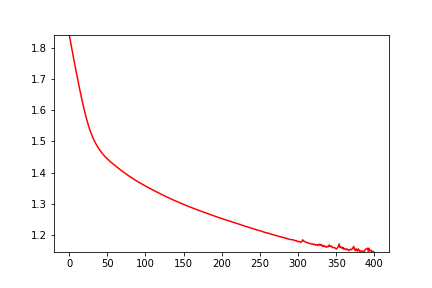
\includegraphics[scale=0.5]{loss-95.png}
		\caption{左图:citeseer链路预测loss曲线,右图:citeseer节点分类loss曲线}
	\end{figure}
\end{document}

